% \begin{wrapfigure}{r}{0.6\linewidth}
\begin{figure}[bt!]
	\centering
\resizebox{1.\linewidth}{!}{
\renewcommand{\arraystretch}{0.5}
\begin{tabular}{@{}c@{\hskip 0.05cm}c@{\hskip 0.05cm}c@{\hskip 0.05cm}c@{}}
		\space
            &
		{\huge Input $t_0$}&
		{\huge Tracked $t_0$}&
		{\huge Tracked $t_1$}&
		% {\small Tracked $t_2$}&
		% {\small Tracked $t_3$}\\

   %           \rotatebox[origin=c]{90}{{\large  Similar colored cars}}&
		 % \raisebox{-0.5\height}{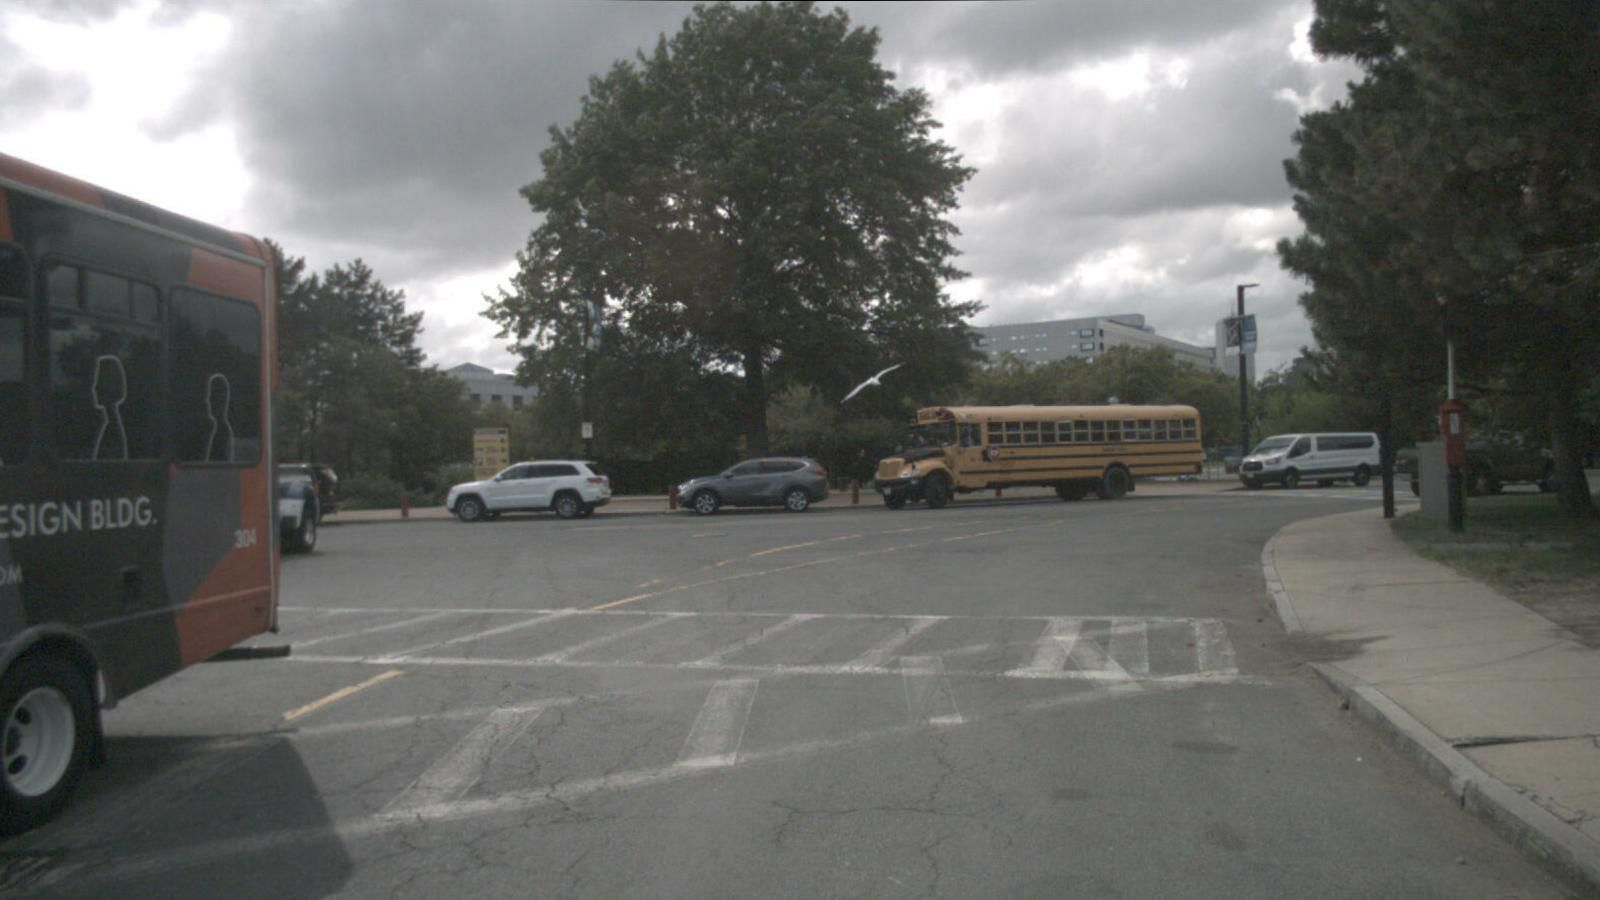
\includegraphics[width=.38\columnwidth, trim={0cm 0cm 0cm 0cm},clip]{fig/additional_nuscenes_results/scene1/26_gt.png}}&
		 % \raisebox{-0.5\height}{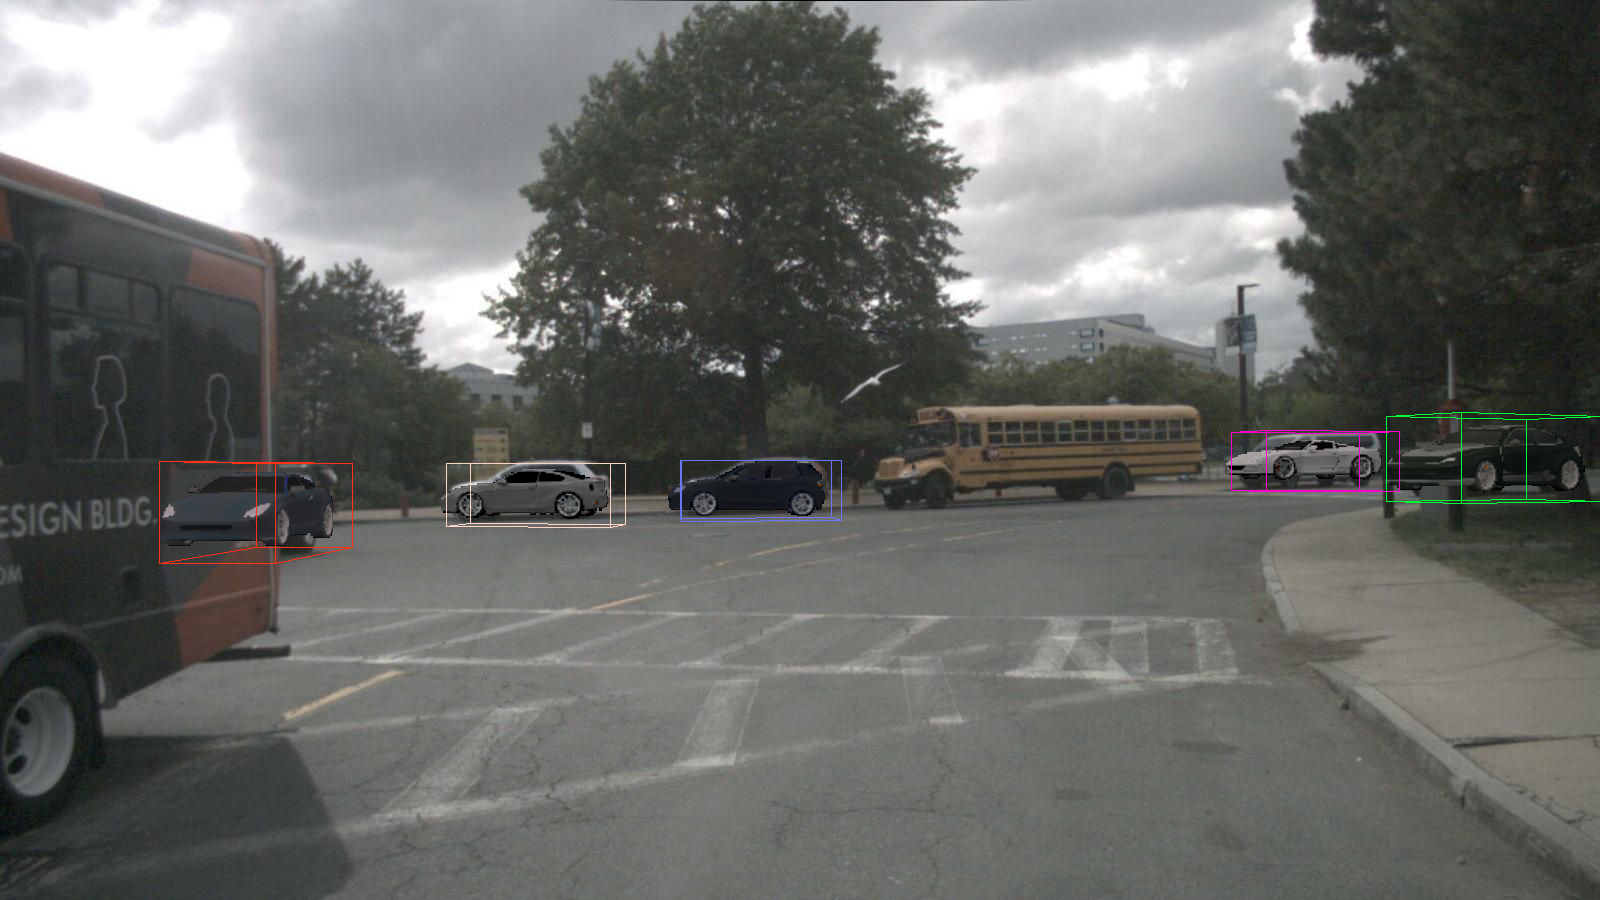
\includegraphics[width=.38\columnwidth, trim={0cm 0cm 0cm 0cm},clip]{fig/additional_nuscenes_results/scene1/26_bbox.png}}&
		 % \raisebox{-0.5\height}{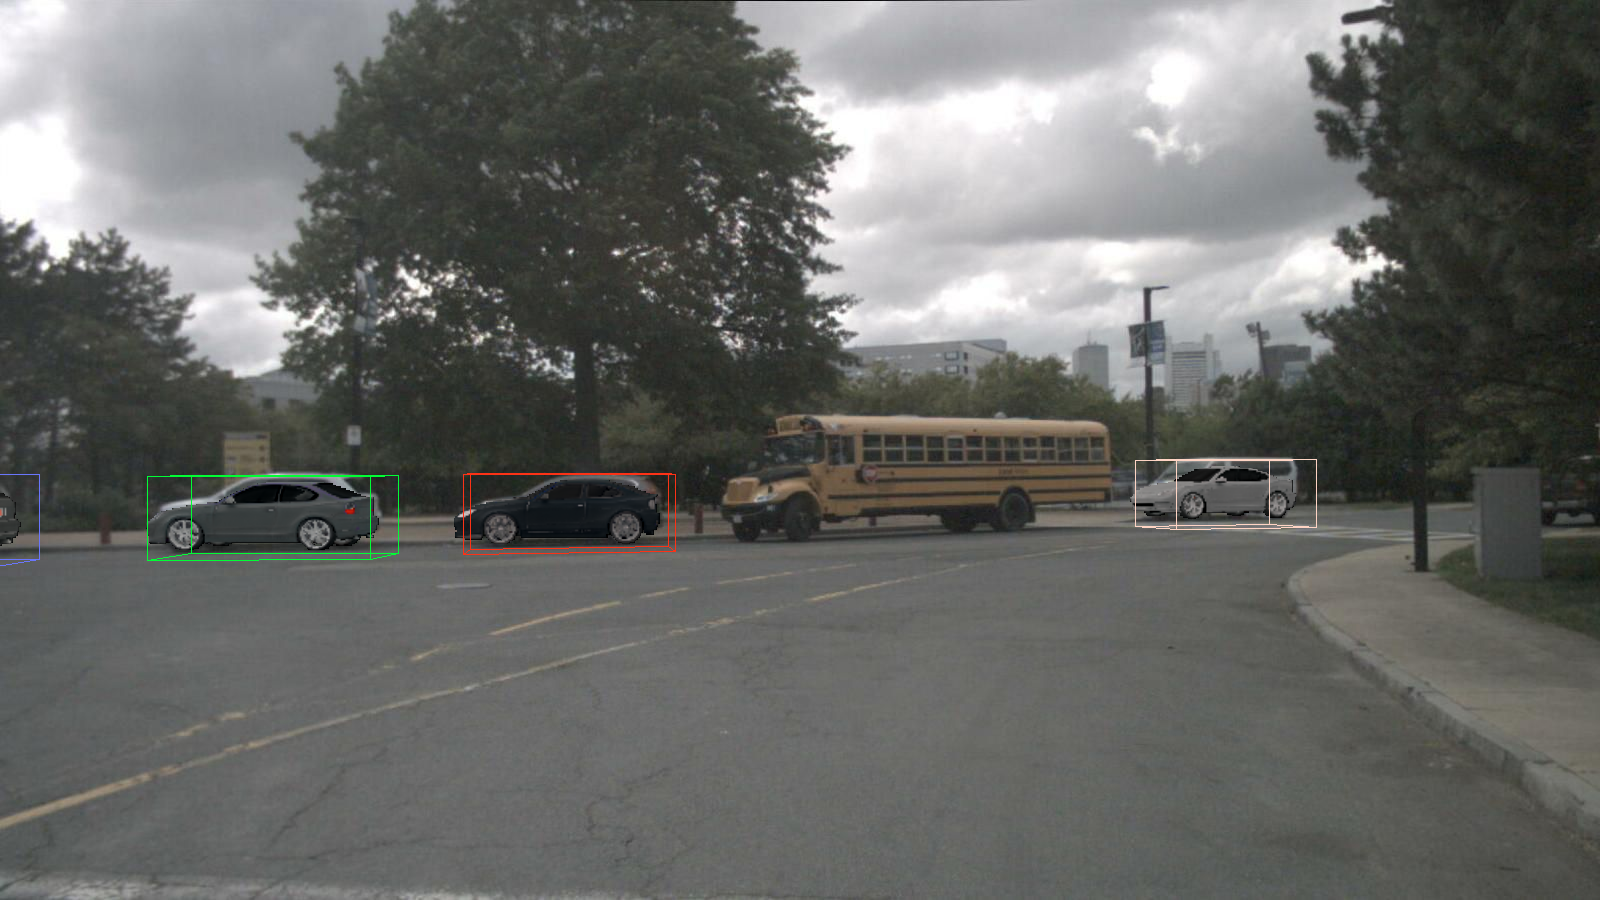
\includegraphics[width=.38\columnwidth, trim={0cm 0cm 0cm 0cm},clip]{fig/additional_nuscenes_results/scene1/28_bbox.png}}&
		 % \raisebox{-0.5\height}{
\includegraphics[width=.38\columnwidth, trim={0cm 0cm 0cm 0cm},clip]{fig/placeholder-img.png}}&
		 % \raisebox{-0.5\height}{
\includegraphics[width=.38\columnwidth, trim={0cm 0cm 0cm 0cm},clip]{fig/placeholder-img.png}}\\[0.95cm]

           \rotatebox[origin=c]{90}{{\Large \textbf{(a)} Shadow}}&
  		\raisebox{-0.5\height}{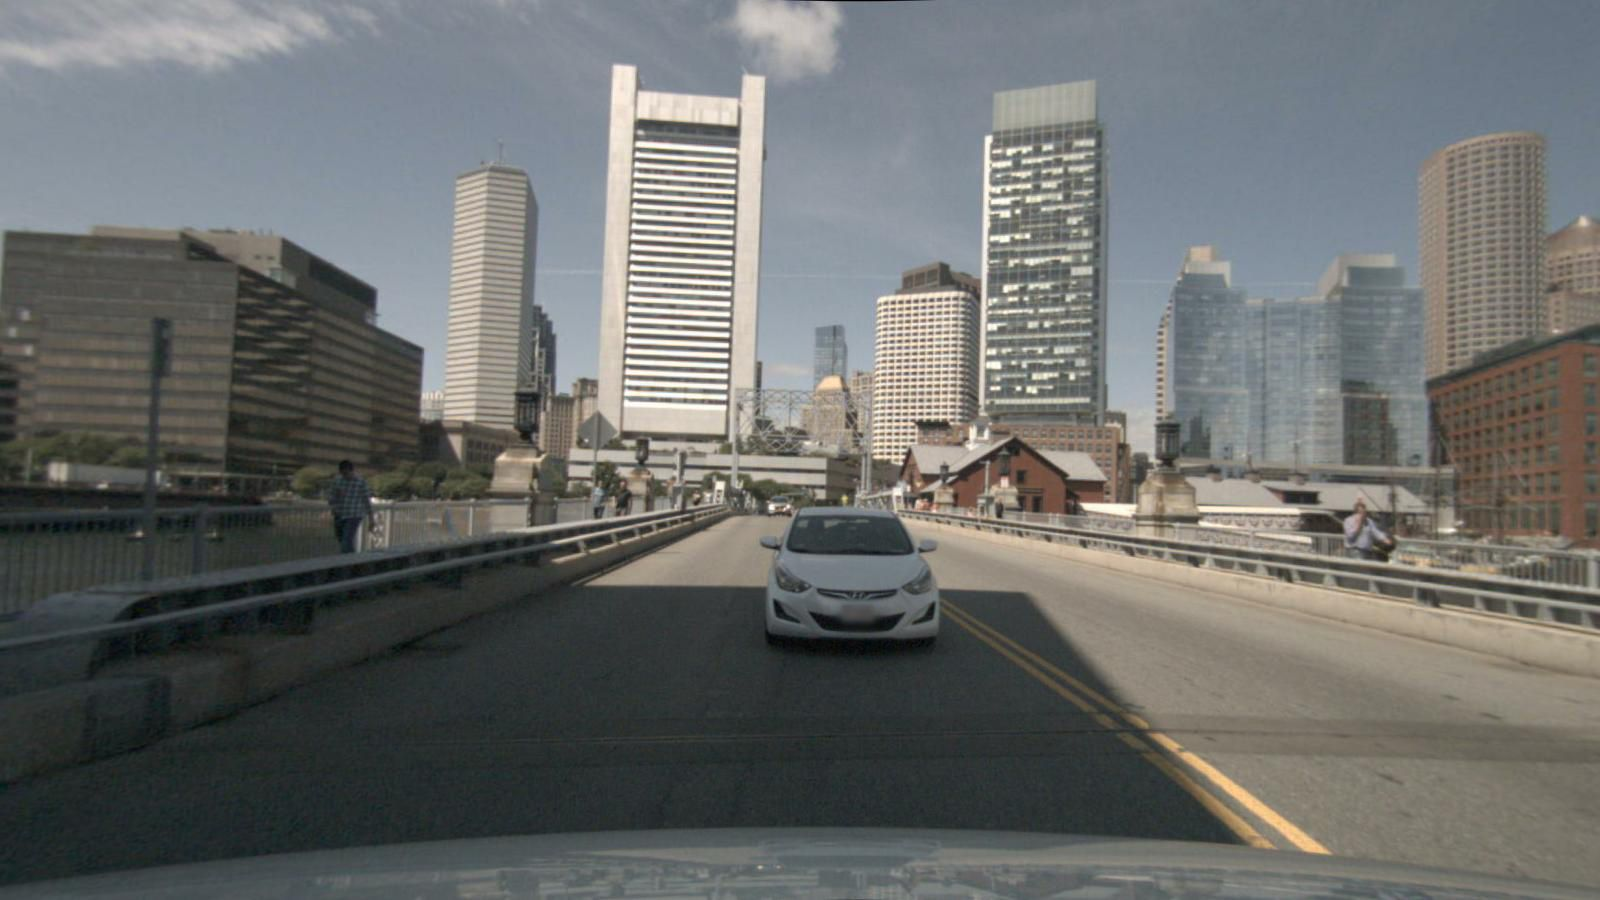
\includegraphics[width=.7\columnwidth, trim={0cm 0cm 0cm 0cm},clip]{fig/additional_nuscenes_results/scene12/gt.png}}&
		\raisebox{-0.5\height}{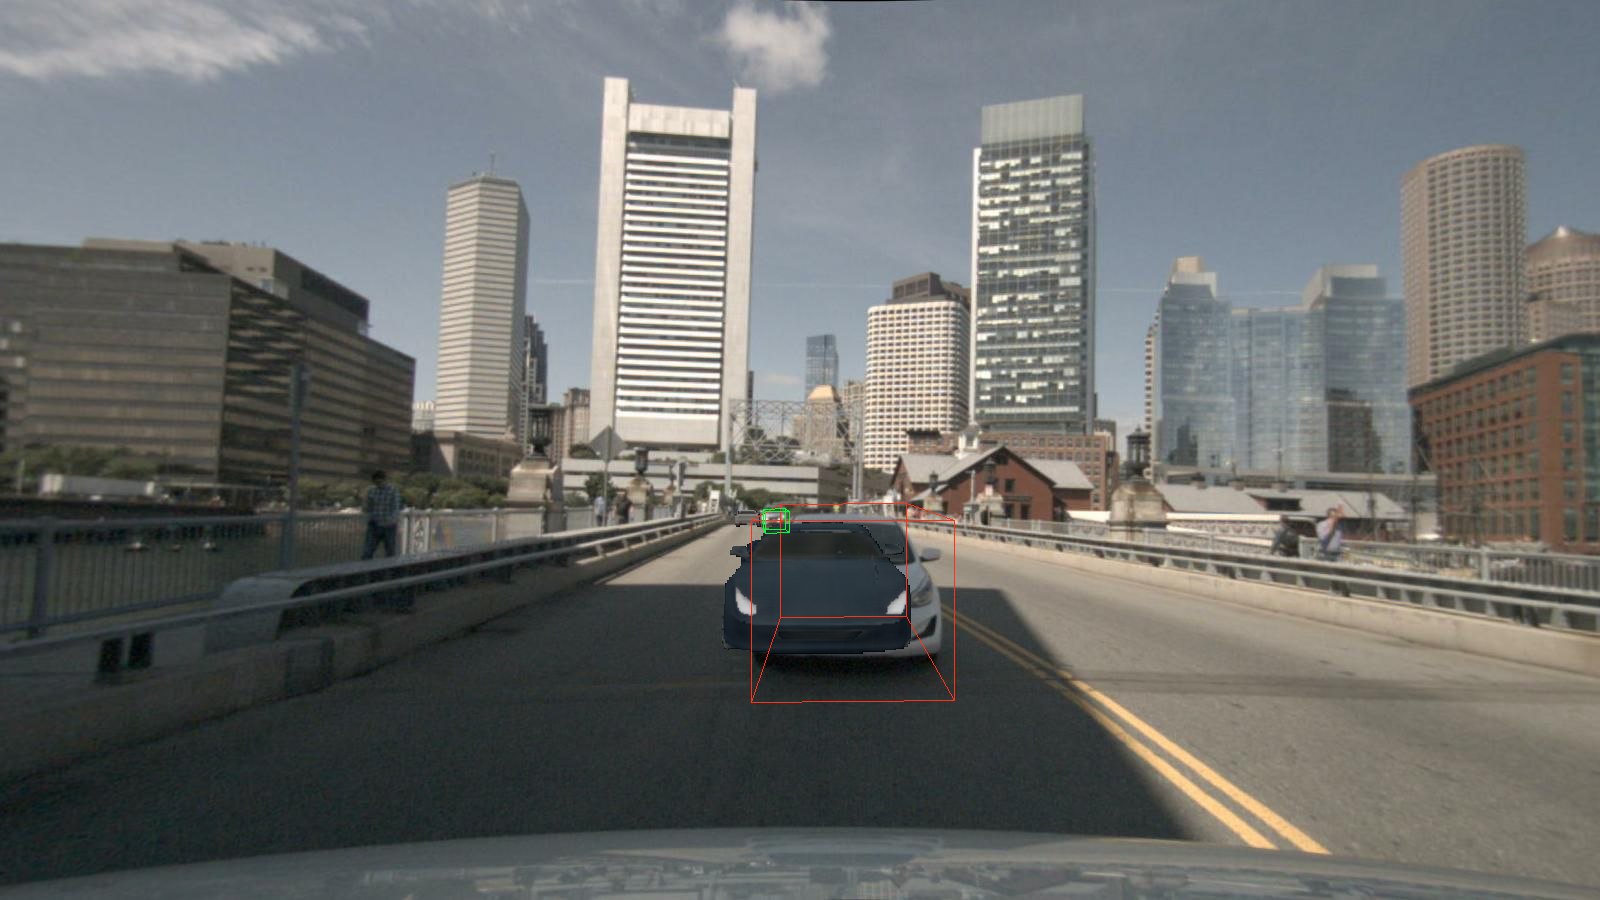
\includegraphics[width=.7\columnwidth, trim={0cm 0cm 0cm 0cm},clip]{fig/additional_nuscenes_results/scene12/21.png}}&
		\raisebox{-0.5\height}{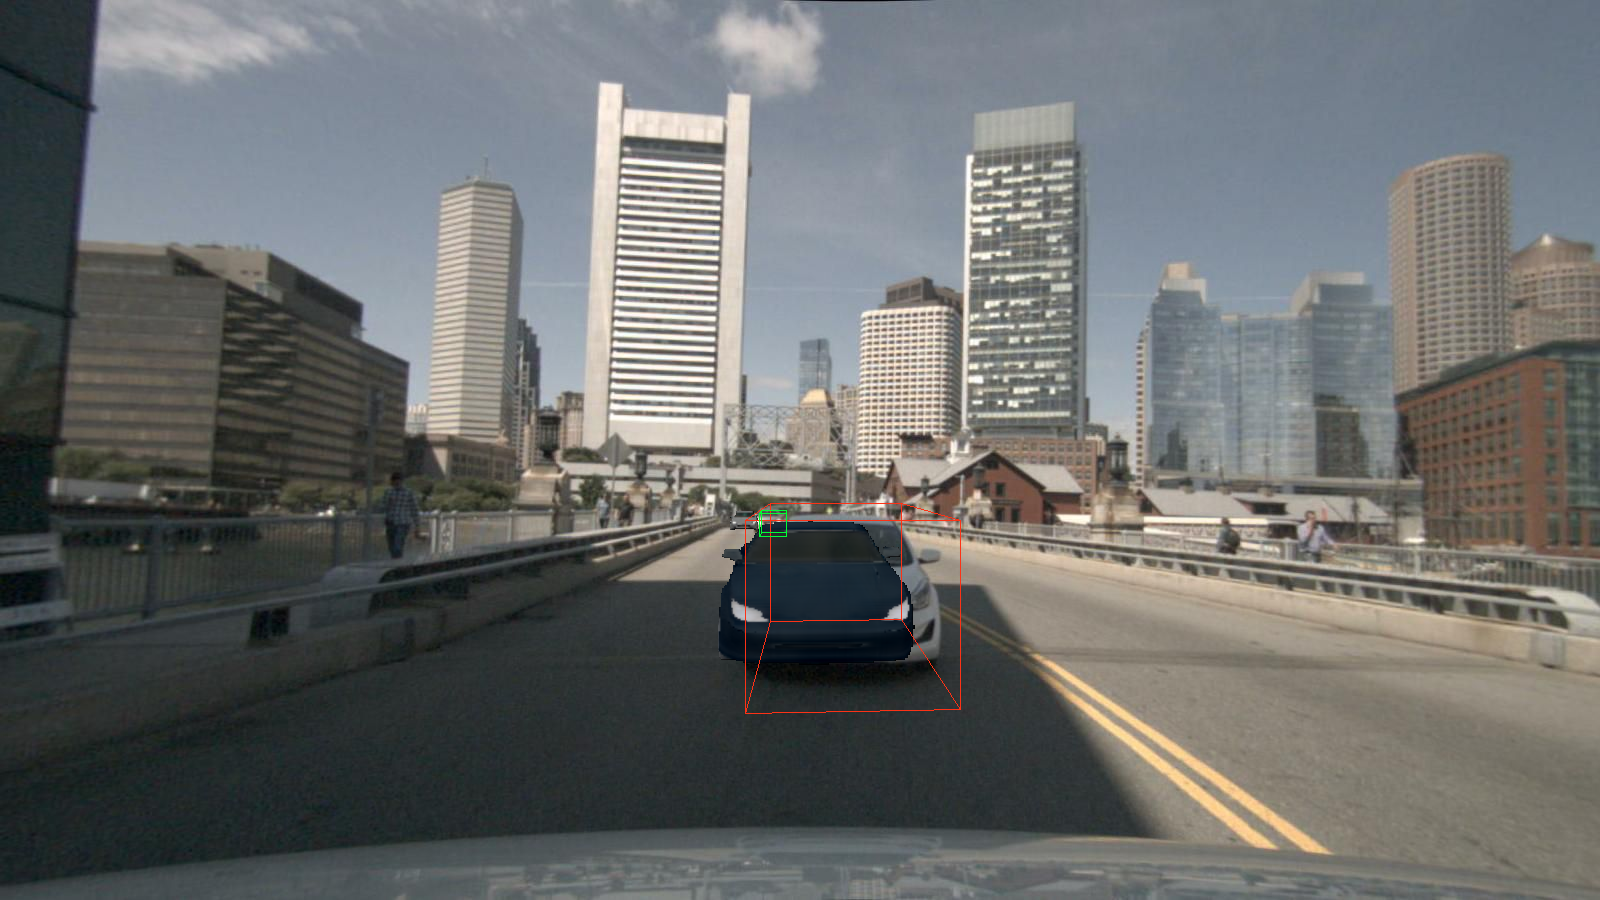
\includegraphics[width=.7\columnwidth, trim={0cm 0cm 0cm 0cm},clip]{fig/additional_nuscenes_results/scene12/22.png}}&
		% \raisebox{-0.5\height}{
\includegraphics[width=.38\columnwidth, trim={0cm 0cm 0cm 0cm},clip]{fig/placeholder-img.png}}&
		% \raisebox{-0.5\height}{
\includegraphics[width=.38\columnwidth, trim={0cm 0cm 0cm 0cm},clip]{fig/placeholder-img.png}}
  \\[0.02cm]

            \rotatebox[origin=c]{90}{{\Large \textbf{(b)} Reflection}}&
  		\raisebox{-0.5\height}{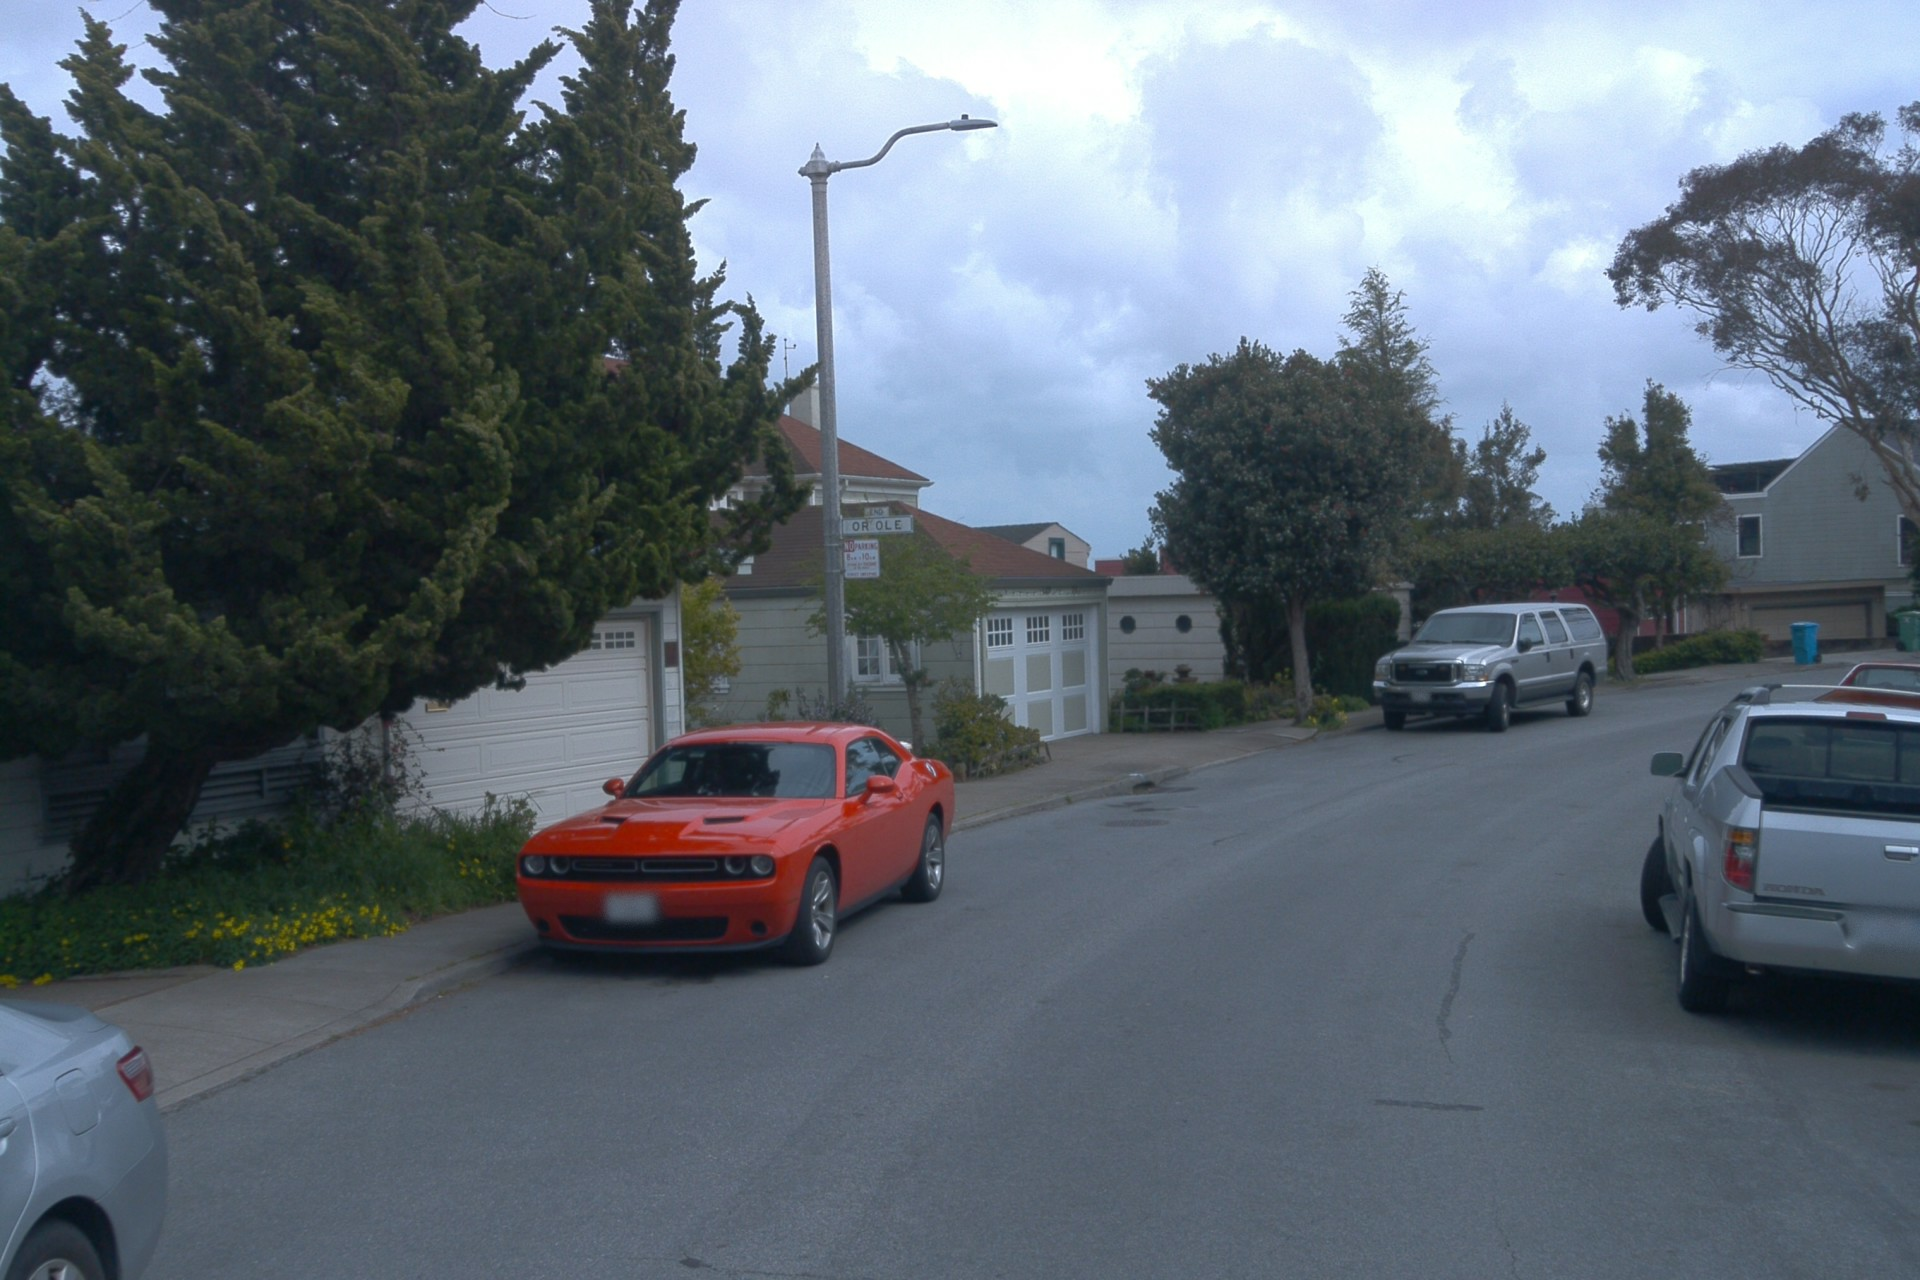
\includegraphics[width=.7\columnwidth, trim={0cm 0cm 0cm 0cm},clip]{fig/additional_waymo_results/scene4/gt_img.png}}&
		\raisebox{-0.5\height}{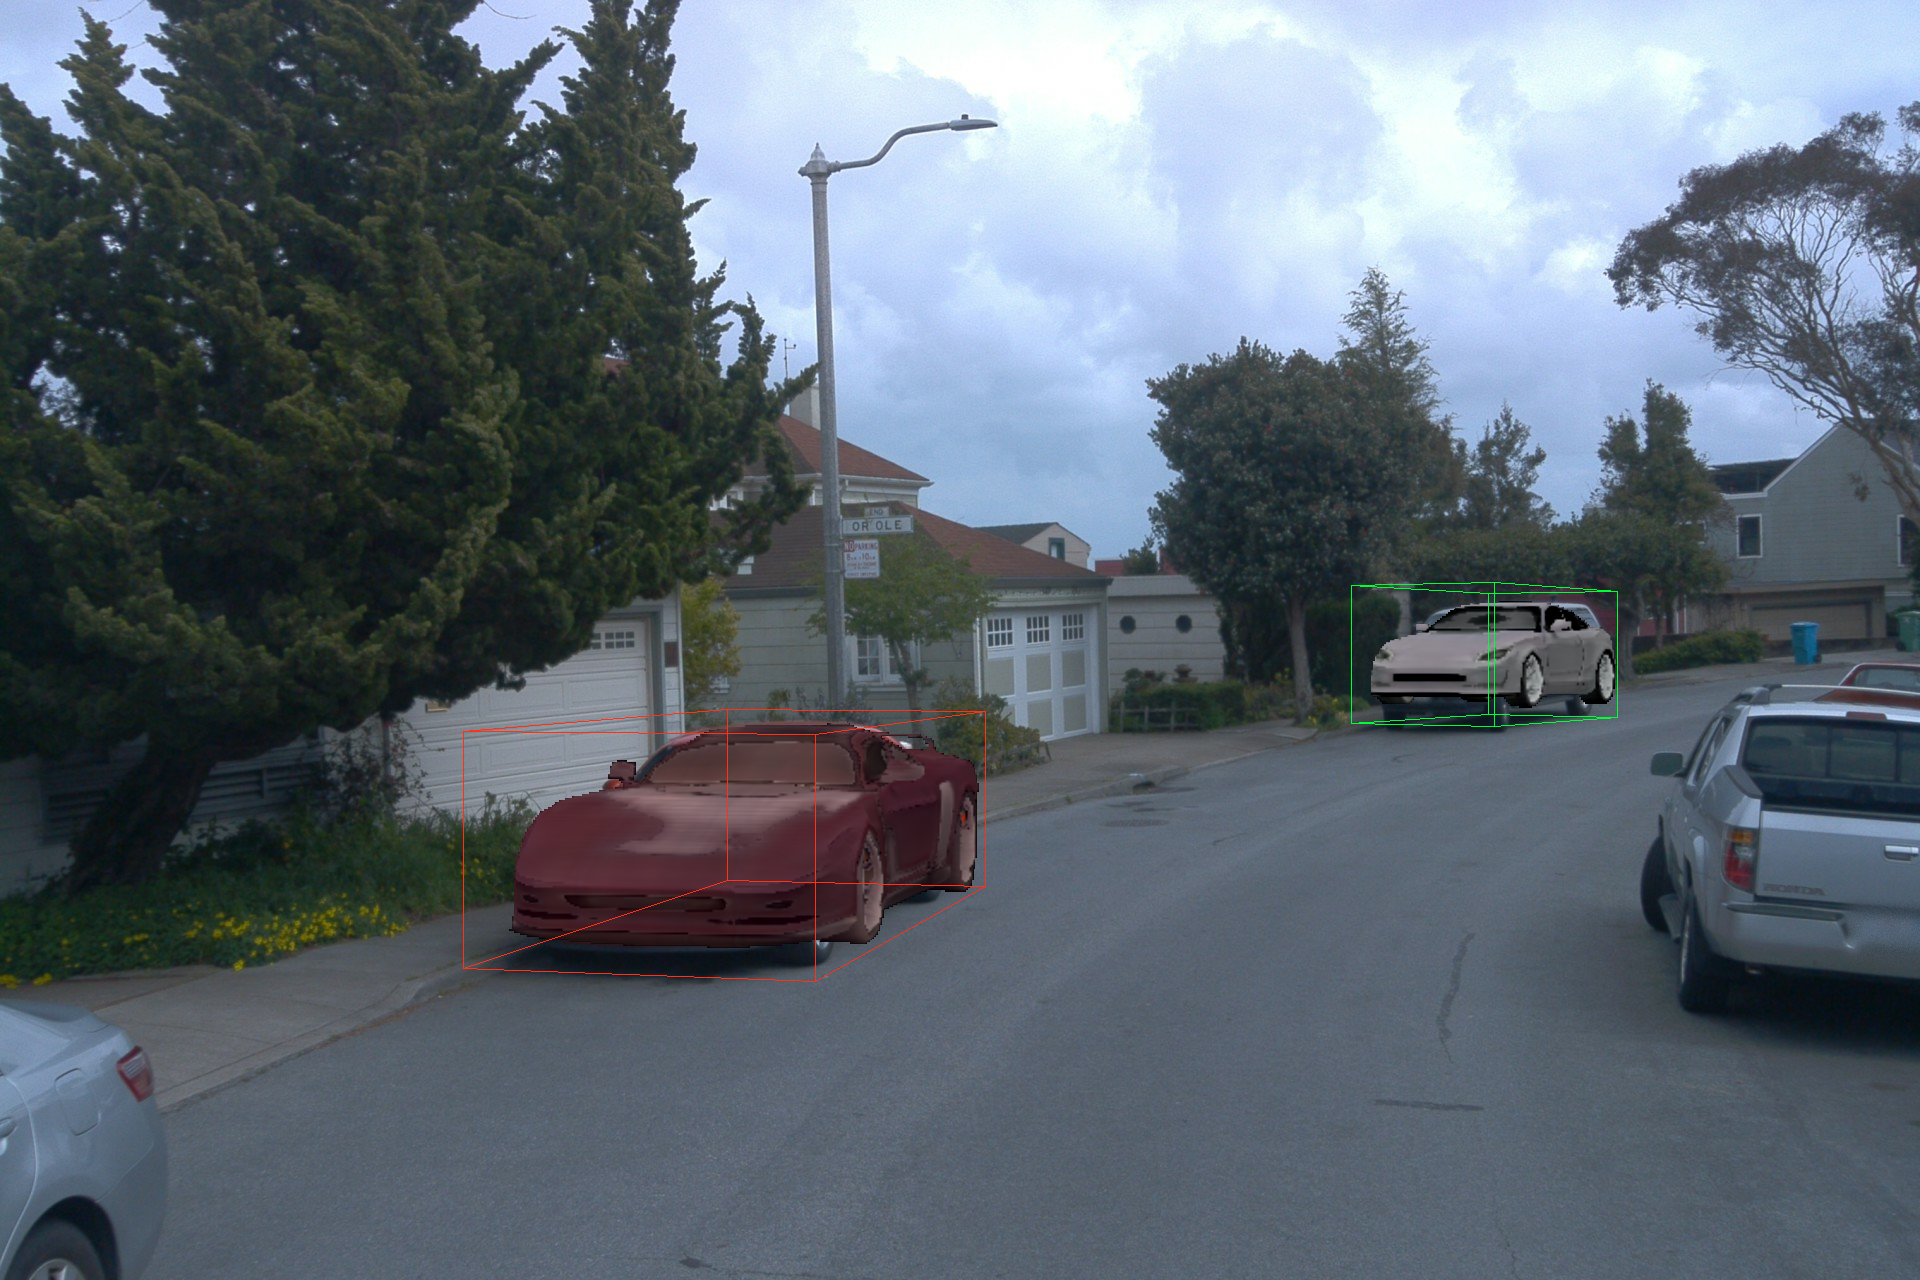
\includegraphics[width=.7\columnwidth, trim={0cm 0cm 0cm 0cm},clip]{fig/additional_waymo_results/scene4/5.png}}&
		\raisebox{-0.5\height}{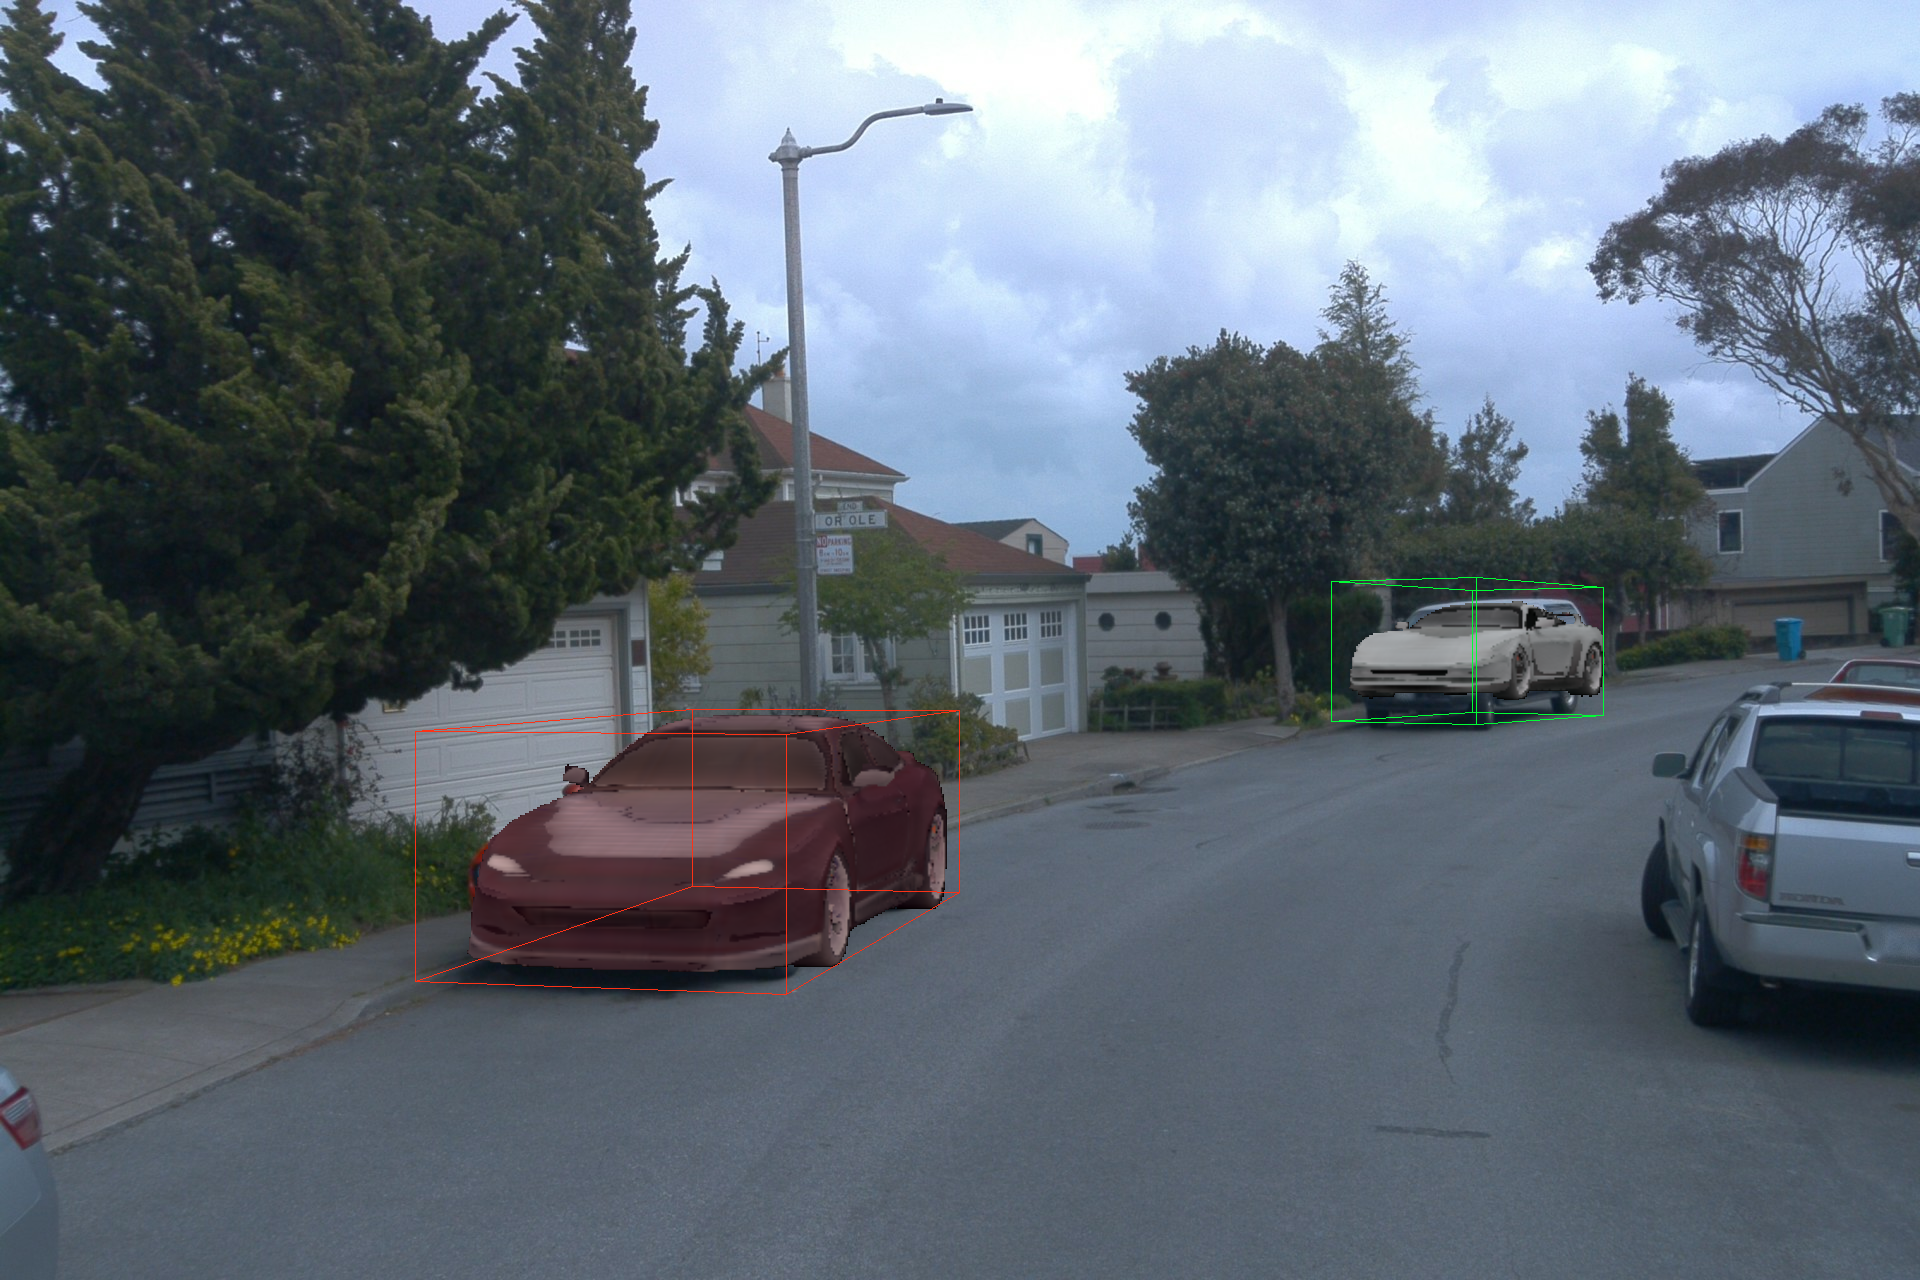
\includegraphics[width=.7\columnwidth, trim={0cm 0cm 0cm 0cm},clip]{fig/additional_waymo_results/scene4/6.png}}&
		% \raisebox{-0.5\height}{
\includegraphics[width=.38\columnwidth, trim={0cm 0cm 0cm 0cm},clip]{fig/placeholder-img.png}}&
		% \raisebox{-0.5\height}{
\includegraphics[width=.38\columnwidth, trim={0cm 0cm 0cm 0cm},clip]{fig/placeholder-img.png}}
  \\[0.02cm]
  
           \rotatebox[origin=c]{90}{{\Large \textbf{(c)} Occlusion}}&
		 \raisebox{-0.5\height}{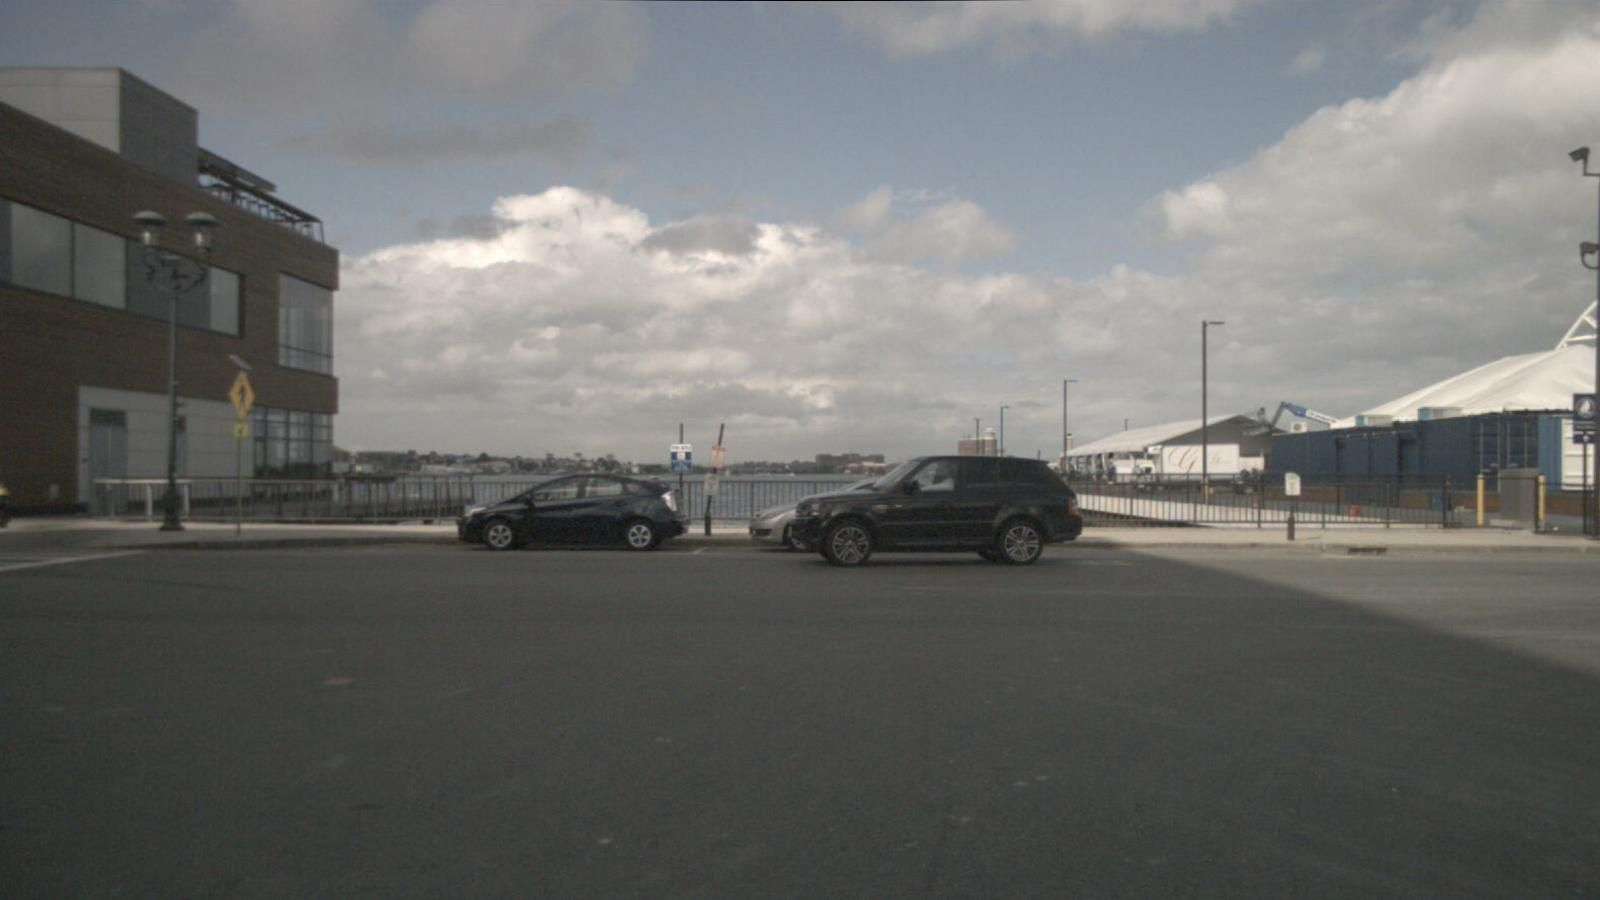
\includegraphics[width=.7\columnwidth, trim={0cm 0cm 0cm 0cm},clip]{fig/additional_nuscenes_results/scene7/0118_4_gt.png}}&
		 \raisebox{-0.5\height}{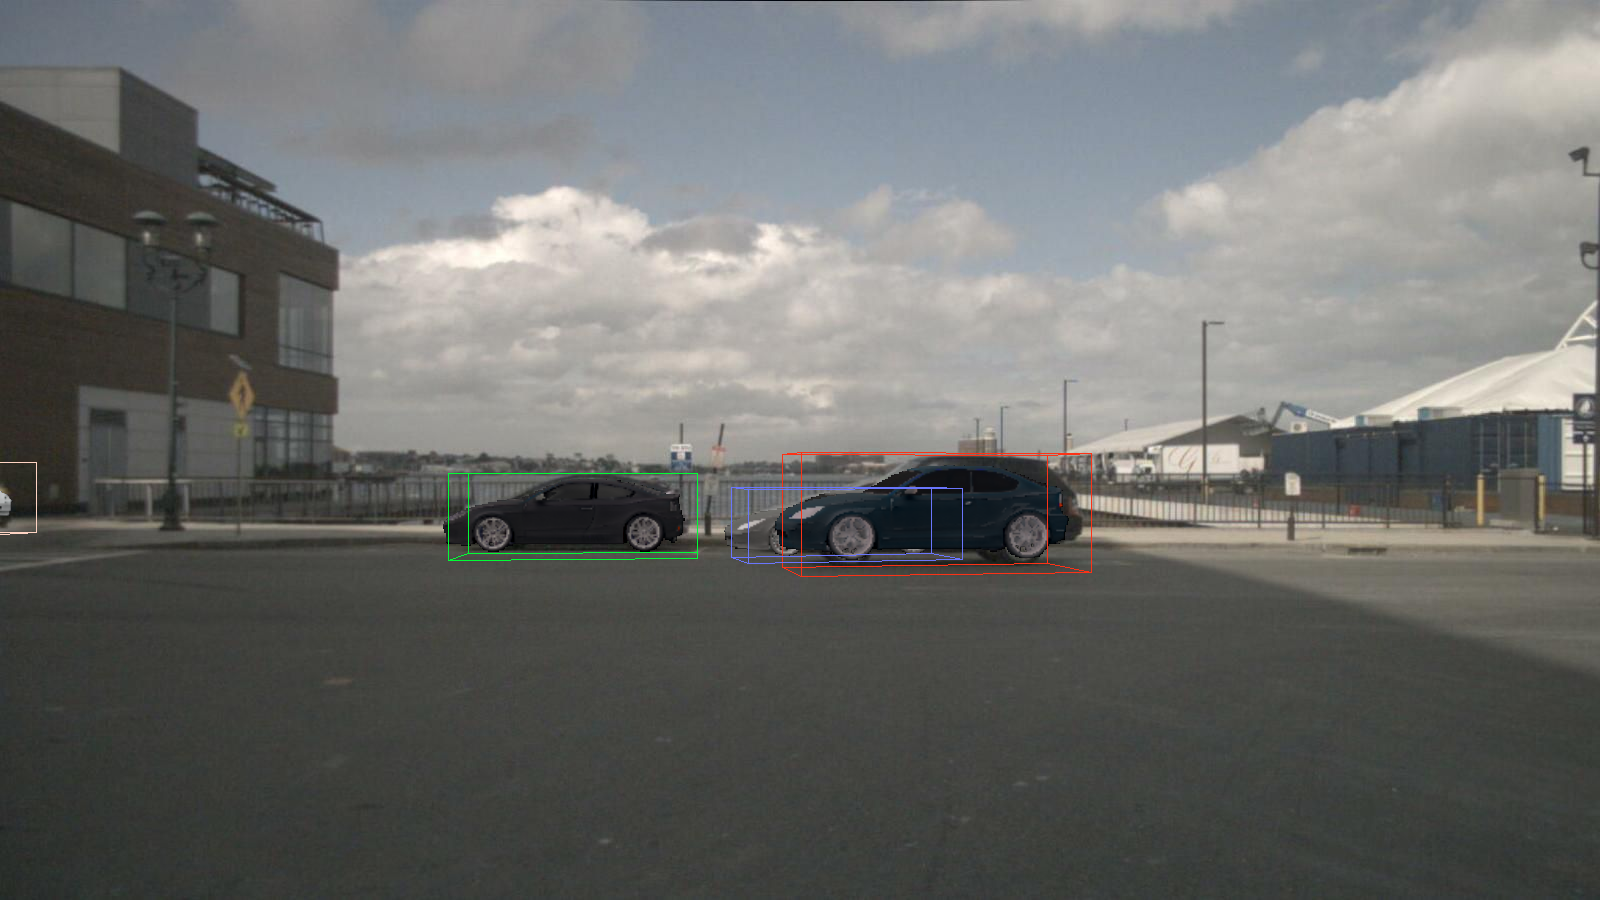
\includegraphics[width=.7\columnwidth, trim={0cm 0cm 0cm 0cm},clip]{fig/additional_nuscenes_results/scene7/0118_4_bbox.png}}&
		 \raisebox{-0.5\height}{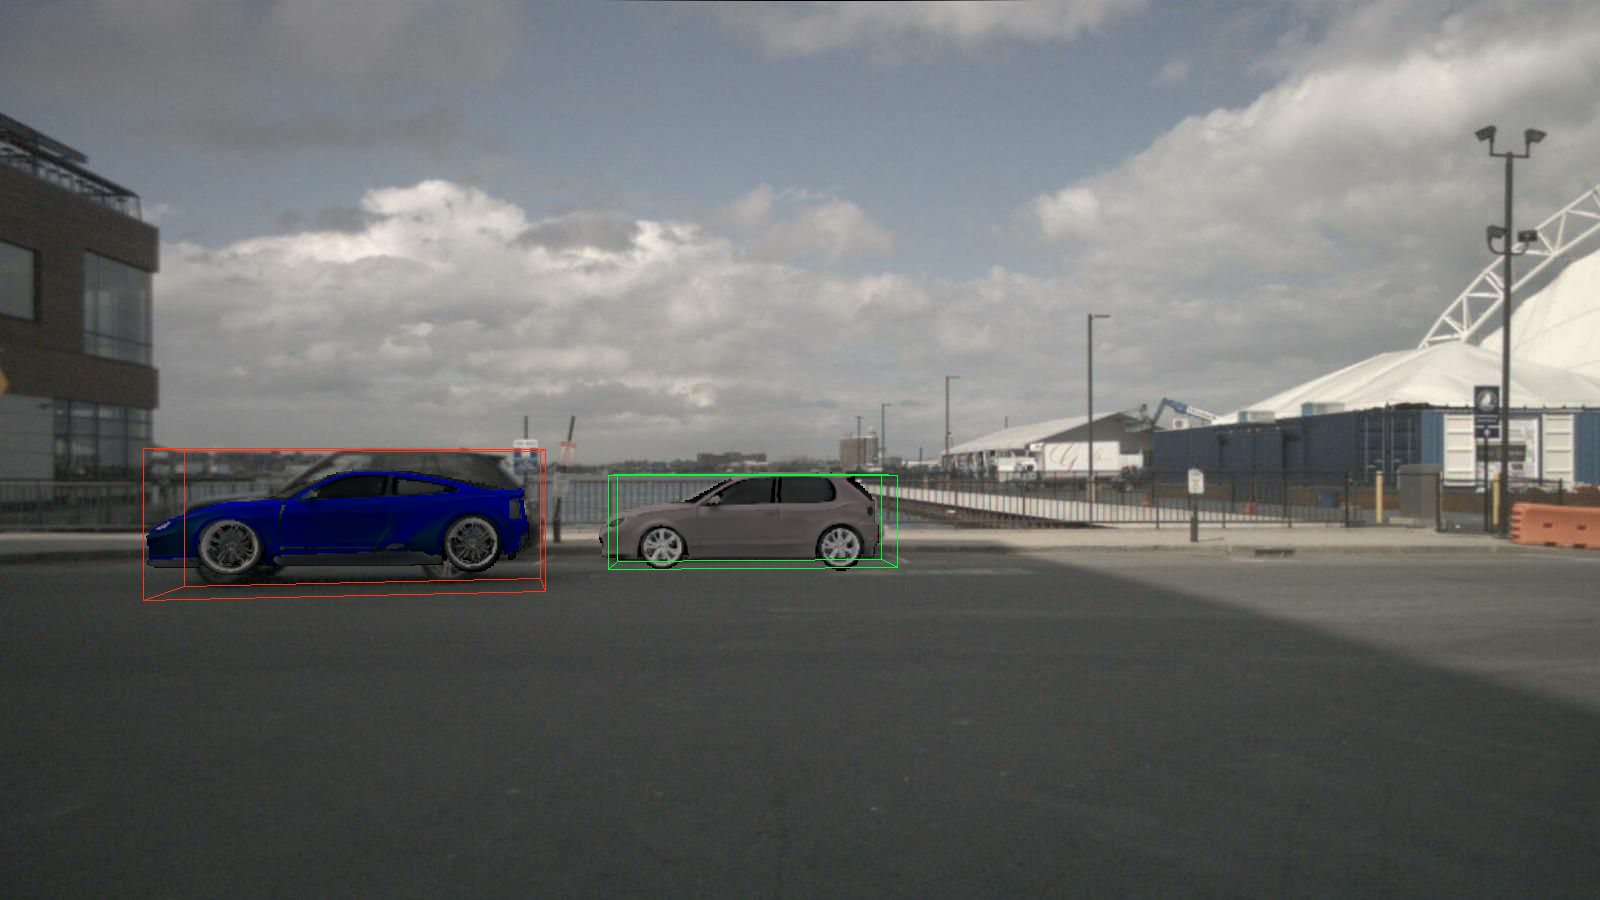
\includegraphics[width=.7\columnwidth, trim={0cm 0cm 0cm 0cm},clip]{fig/additional_nuscenes_results/scene7/0118_6_bbox.png}}&
		 % \raisebox{-0.5\height}{
\includegraphics[width=.38\columnwidth, trim={0cm 0cm 0cm 0cm},clip]{fig/placeholder-img.png}}&
		 % \raisebox{-0.5\height}{
\includegraphics[width=.38\columnwidth, trim={0cm 0cm 0cm 0cm},clip]{fig/placeholder-img.png}}
   \\[0.02cm]
        
        \rotatebox[origin=c]{90}{{\Large \textbf{(d)} Obstruction}}&
		 \raisebox{-0.5\height}{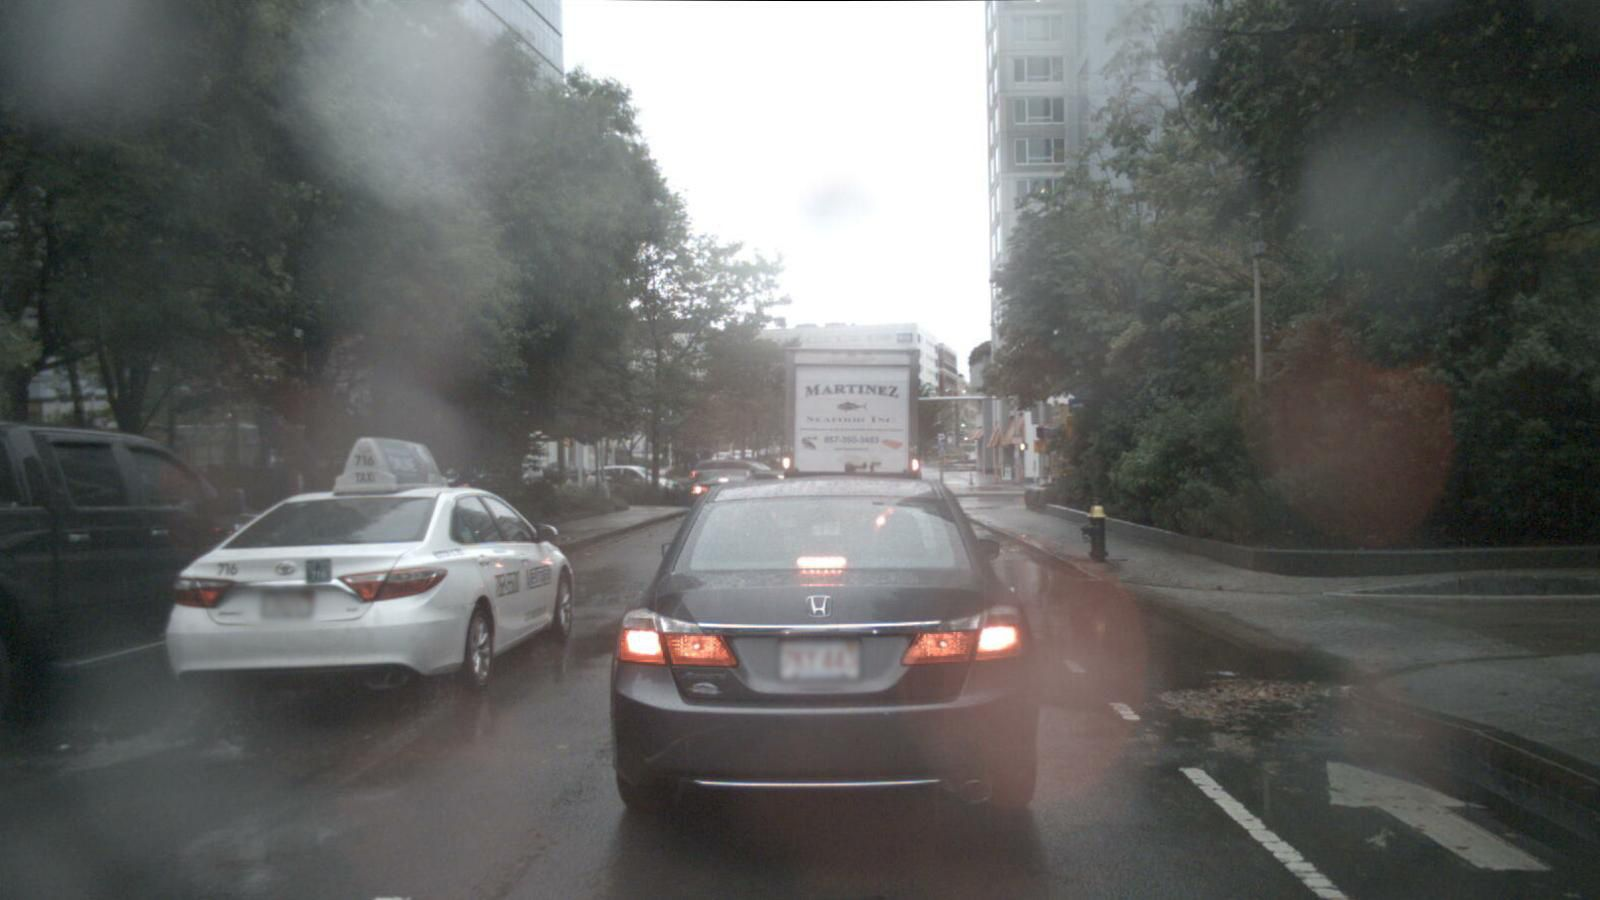
\includegraphics[width=.7\columnwidth, trim={0cm 0cm 0cm 0cm},clip]{fig/additional_nuscenes_results/rainy_scene/gt_img.png}}&
		 \raisebox{-0.5\height}{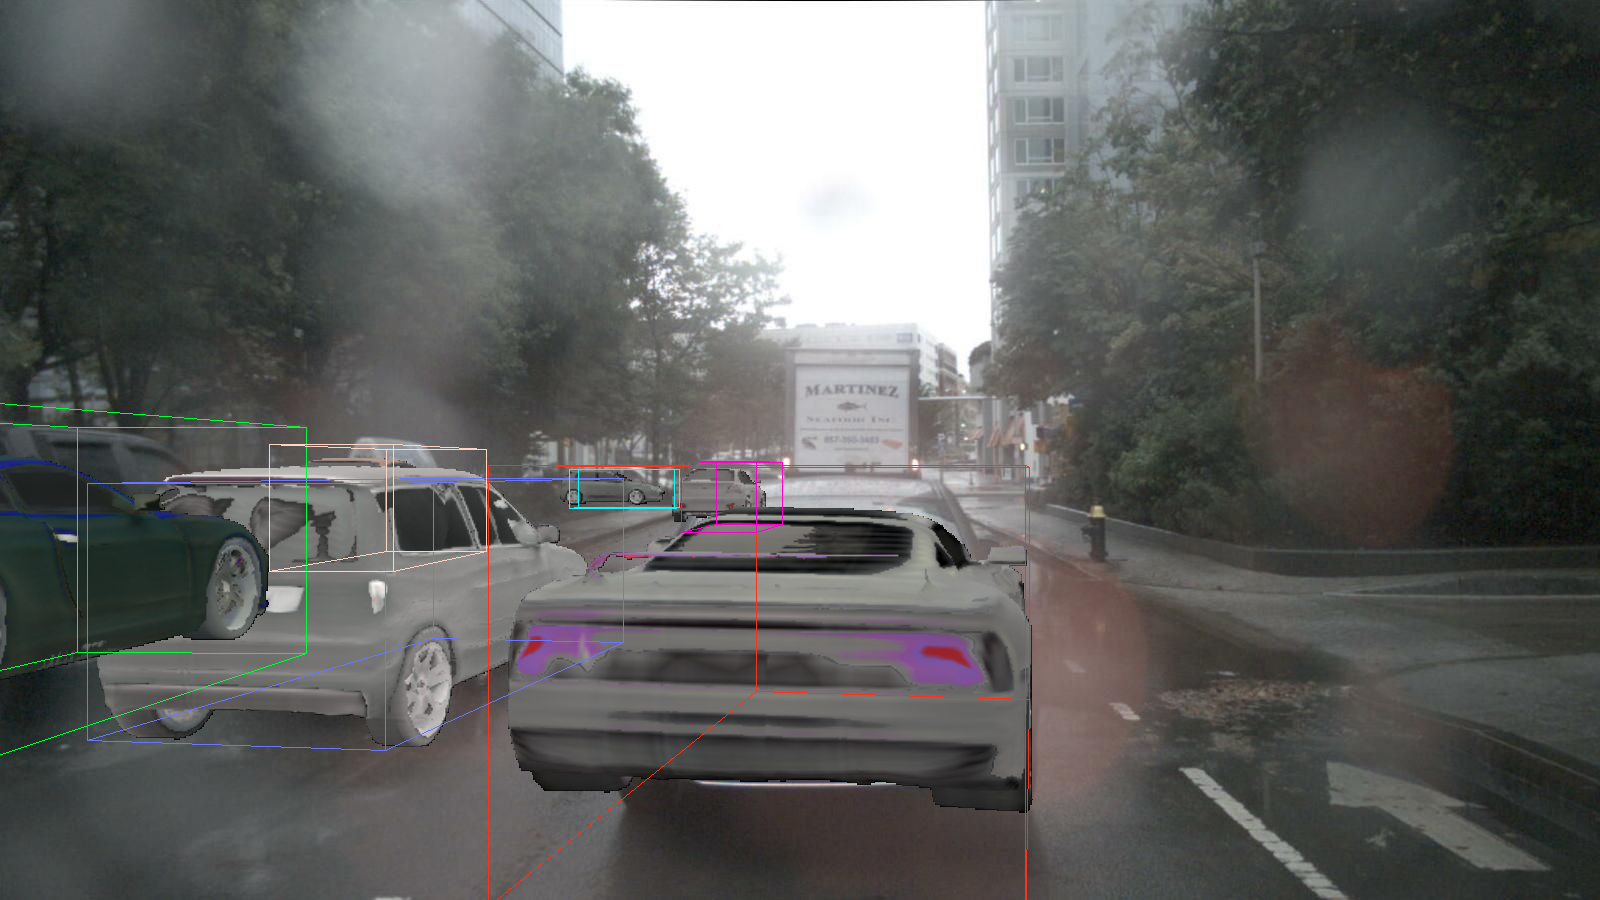
\includegraphics[width=.7\columnwidth, trim={0cm 0cm 0cm 0cm},clip]{fig/additional_nuscenes_results/rainy_scene/30.png}}&
		 \raisebox{-0.5\height}{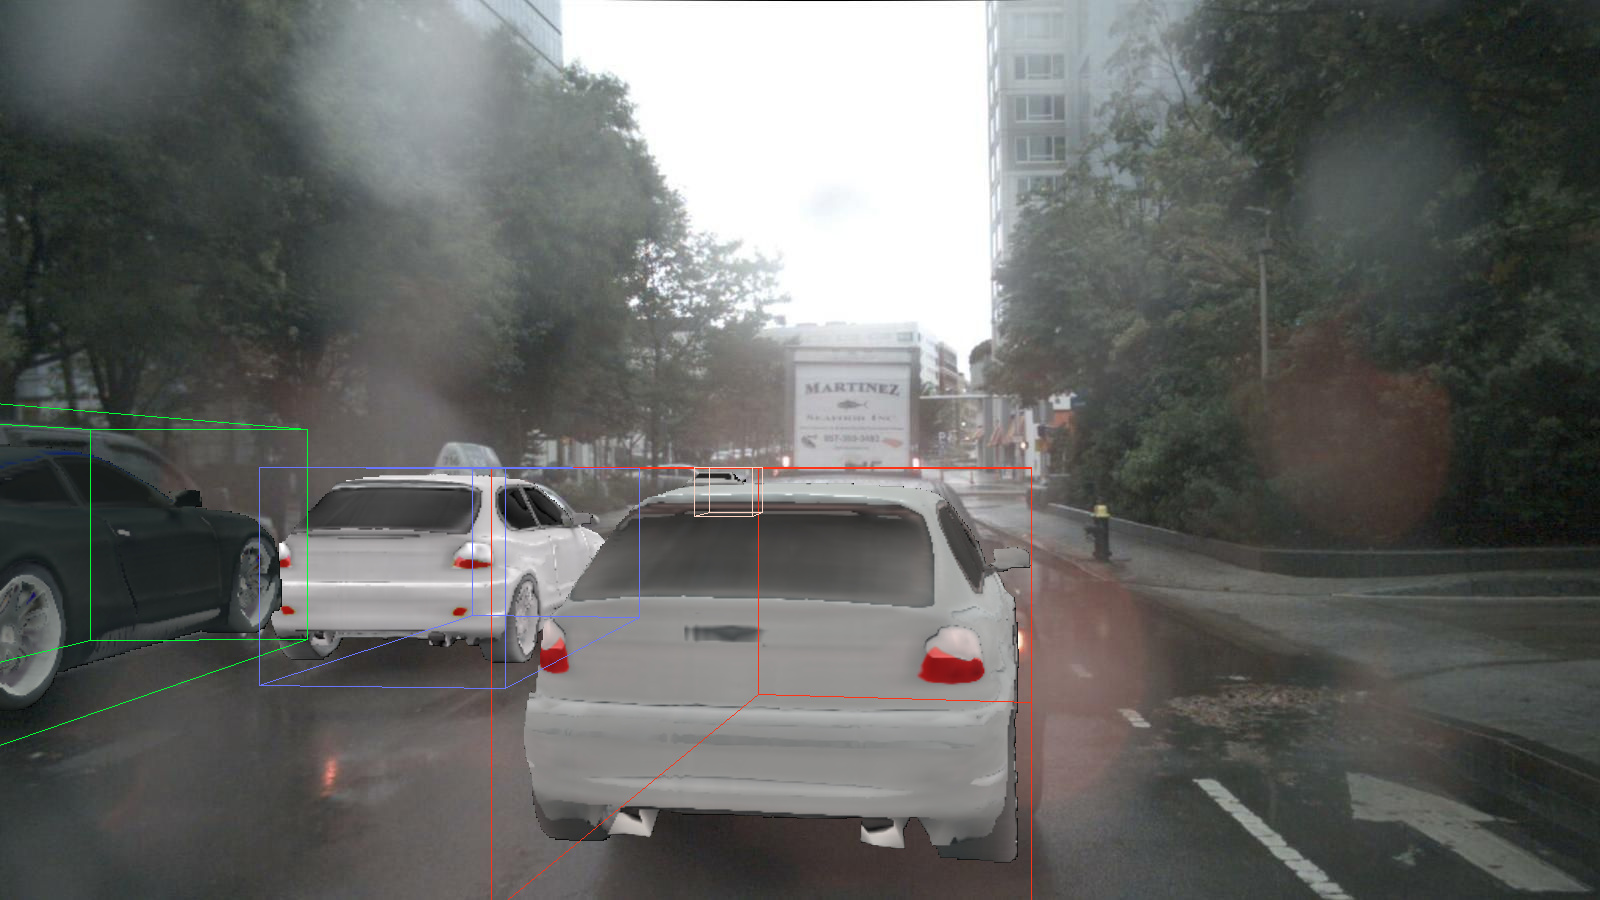
\includegraphics[width=.7\columnwidth, trim={0cm 0cm 0cm 0cm},clip]{fig/additional_nuscenes_results/rainy_scene/31.png}}&
		 % \raisebox{-0.5\height}{
\includegraphics[width=.38\columnwidth, trim={0cm 0cm 0cm 0cm},clip]{fig/placeholder-img.png}}&
		 % \raisebox{-0.5\height}{
\includegraphics[width=.38\columnwidth, trim={0cm 0cm 0cm 0cm},clip]{fig/placeholder-img.png}}
   \\[0.02cm]

   		\rotatebox[origin=c]{90}{{\Large \textbf{(e)} Det. Accuracy}}&
		\raisebox{-0.5\height}{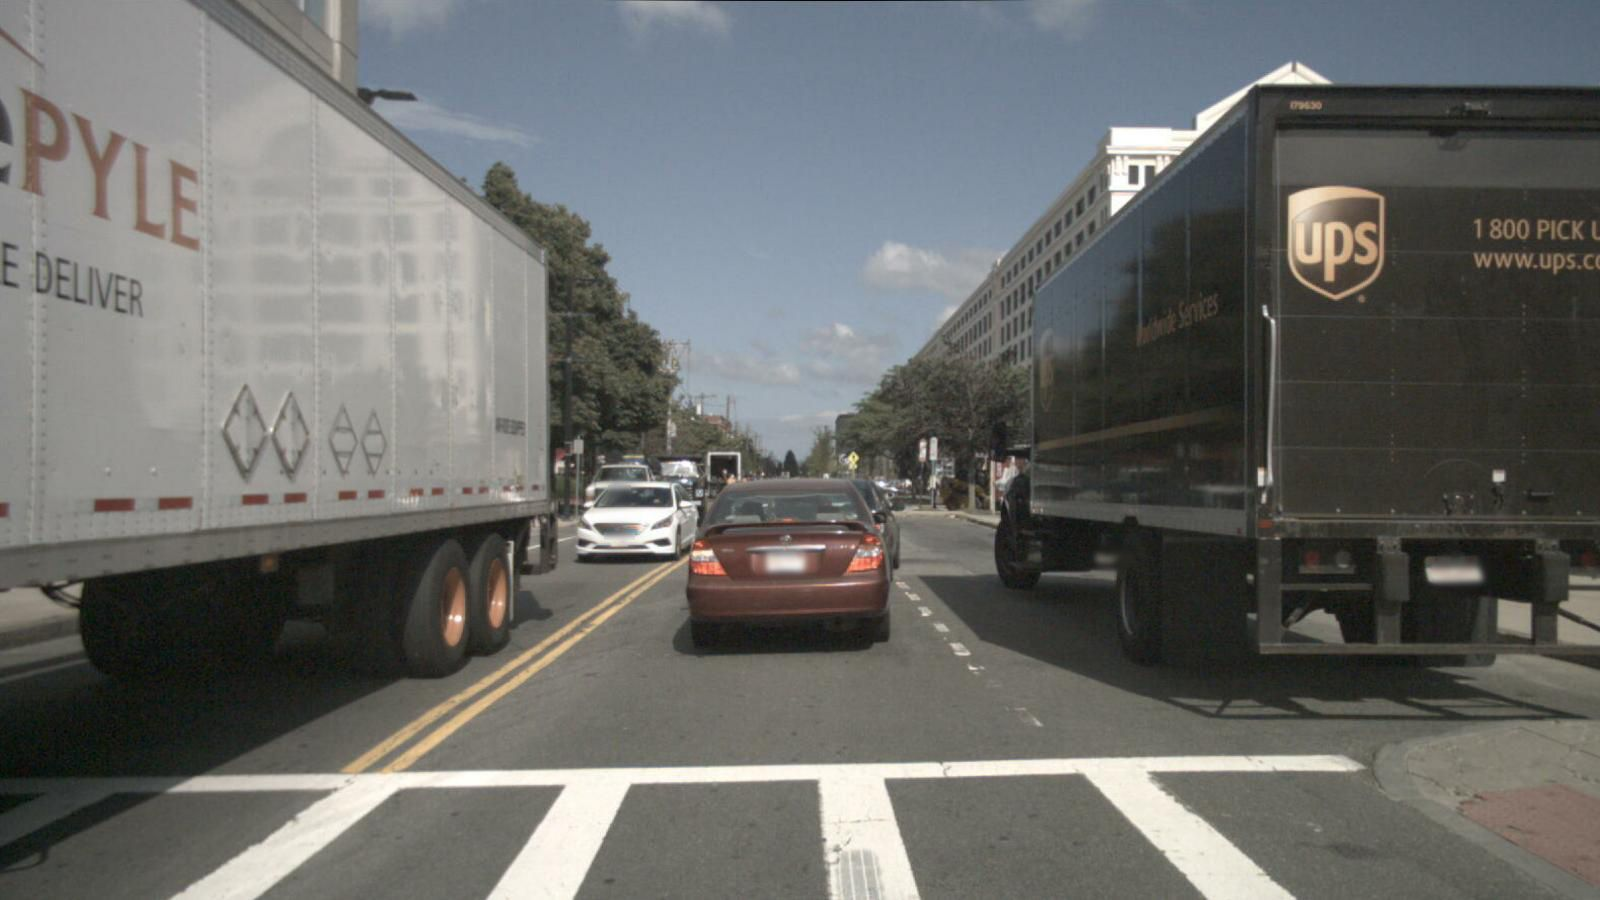
\includegraphics[width=.7\columnwidth, trim={0cm 0cm 0cm 0cm},clip]{fig/additional_nuscenes_results/scene2/2_gt.png}}&
		\raisebox{-0.5\height}{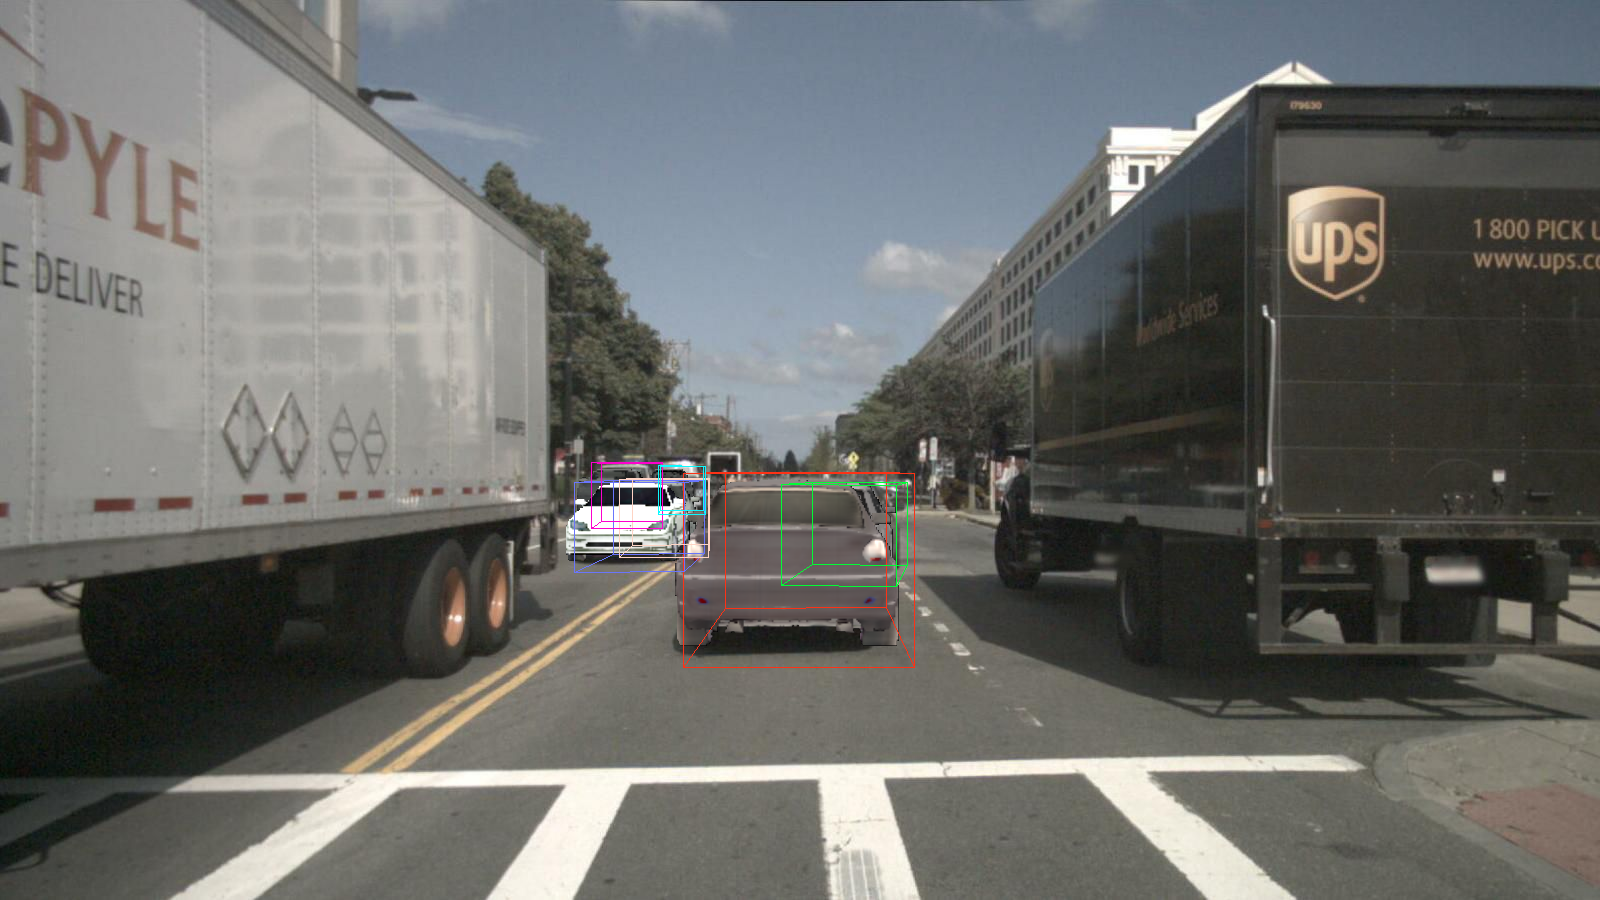
\includegraphics[width=.7\columnwidth, trim={0cm 0cm 0cm 0cm},clip]{fig/additional_nuscenes_results/scene2/2)bbix.png}} &
		\raisebox{-0.5\height}{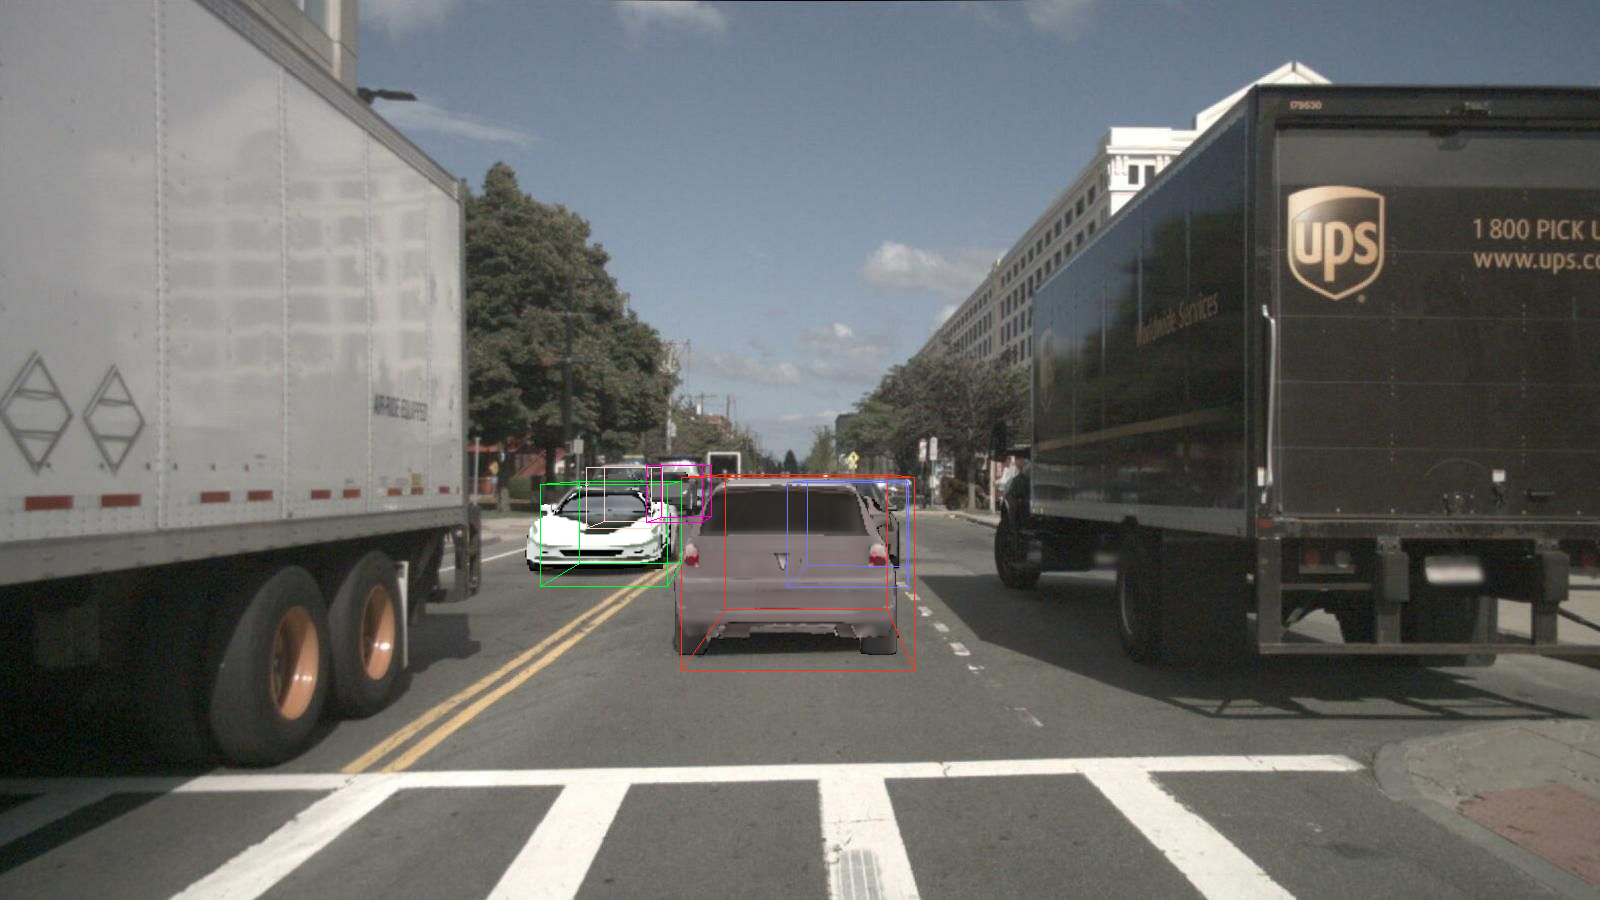
\includegraphics[width=.7\columnwidth, trim={0cm 0cm 0cm 0cm},clip]{fig/additional_nuscenes_results/scene2/3_bbox.png}}&
		% \raisebox{-0.5\height}{
\includegraphics[width=.38\columnwidth, trim={0cm 0cm 0cm 0cm},clip]{fig/placeholder-img.png}}&
		% \raisebox{-0.5\height}{
\includegraphics[width=.38\columnwidth, trim={0cm 0cm 0cm 0cm},clip]{fig/placeholder-img.png}}
\end{tabular}}
\caption{Examples of failure cases, such as lighting (shadows and reflections) or occluded objects, where the reconstructed object differs significantly from the observed object. These visualizations allow us to understand exactly why our model fails at reconstructing and tracking objects. This also allows us to identify ways the representation model and perception pipeline can be improved to incorporate effects that cause the method to fail.}
	\label{fig:interpretability}
 \end{figure}
% \end{wrapfigure}
